\documentclass[a4paper,12pt,titlepage]{article}

% Paquetes
\usepackage[spanish,es-lcroman]{babel}
\usepackage[utf8]{inputenc}
\usepackage{alltt}
\usepackage{verbatim}
%   - minted: Highlighting de código con Pygments
\usepackage{minted}
%   - cleveref: Intelligent cross-referencing
\usepackage{cleveref}
\usepackage{titlesec}
%   - Glosario
\usepackage[hyperfootnotes=false]{hyperref}
\usepackage[nomain,xindy,toc,acronym]{glossaries}
%   - Visual
\usepackage{float}
\usepackage{setspace}
\usepackage{xspace}
\usepackage{xcolor}
\usepackage{graphicx}
\usepackage{amssymb}
\usepackage{amsthm}
\usepackage{tikz}
%   - Índices
\usepackage[xindy]{imakeidx}
%   - Bloques preformateados
\usepackage{listings}

% Configuración
%   - Espacio entre el texto principal y las notas al pie
\setlength{\skip\footins}{1cm}
%   - Espacio entre notas al pie
\setlength{\footnotesep}{0.5cm}
%   - Formatos
% \setmainfont{Droid serif} % Si se desea cambiar la tipografía
\titleformat{\paragraph}
{\normalfont\normalsize\bfseries}{\theparagraph}{1em}{}
\titlespacing*{\paragraph}
{0pt}{3.25ex plus 1ex minus .2ex}{1.5ex plus .2ex}
%   - Resaltado de sintaxis
\setminted{
  fontsize=\small,
  style=colorful % o style=bw para blanco y negro
}
%     + Define el ambiente {phpcode} para código PHP
\newminted{php}{linenos}
%     + Define el comando \phpfile{path} para código PHP desde archivos externos
\newmintedfile{php}{linenos}
%     + Define el ambiente {rubycode} para código Ruby
\newminted{ruby}{linenos}
%     + Define el comando \rubyfile{path} para código ruby desde archivos externos
\newmintedfile{ruby}{linenos}
%     + Define el ambiente {bashcode} para comandos de CLI
\newminted{bash}{}
%     + Define el comando \bashfile{path} para comandos de CLI desde archivos externos
\newmintedfile{bash}{}
%     + Define el ambiente {jsoncode} para código JSON
\newminted{json}{}
%     + Define el comando \jsonfile{path} para código JSON desde archivos externos
\newmintedfile{json}{}
%     + Define el ambiente {httpcode} para sesiones HTTP
\newminted{http}{linenos}
%     + Define el comando \httpfile{path} para sesiones HTTP desde archivos externos
\newmintedfile{http}{}
%   - Formato de los glosarios
\setglossarystyle{altlist}
%   - Formato de bloques preformateados
\lstset{
  basicstyle=\small\ttfamily,
  columns=flexible,
  breaklines=true
}
%   - Formato de los \subparagraphs para que tengan un salto de línea que los separe del texto
\titleformat{\subparagraph}{\normalfont\normalsize\bfseries}{\thesubparagraph}{1em}{}
\titlespacing*{\subparagraph}{\parindent}{3.25ex plus 1ex minus .2ex}{.75ex plus .1ex}
%   - Nombre y título para los bloques de código de minted
\renewcommand{\listingscaption}{Bloque de código}
\renewcommand{\listoflistingscaption}{Listado de bloques de código}

% Definición de ambientes
%   - displaycode: para mostrar código
\newenvironment{displaycode}{\begin{alltt}}{\end{alltt}}
%   - code: para mostrar código
%\newenvironment{code}{\color{Sepia}\verbatim}{\endverbatim}
\newenvironment{code}{\verbatim}{\endverbatim}

% Comandos personalizados

% {\fechaPresentacion} :: para escribir la fecha de presentación del trabajo
\newcommand{\fechaPresentacion}{\today}
% {\unlp} :: para escribir "Universidad Nacional de La Plata"
\newcommand{\unlp}{Universidad Nacional de La Plata}
% {\facultad} :: para escribir "Facultad de Informática"
\newcommand{\facultad}{Facultad de Informática}
% {\cespi} :: para escribir "CeSPI"
\newcommand{\cespi}{CeSPI}
% {\direccionDesarrollo} :: Para escribir "Dirección de Desarrollo del CeSPI"
\newcommand{\direccionDesarrollo}{Dirección de Desarrollo del {\cespi}}
% {\tituloTrabajo} :: Para escribir el título de la tesina
\newcommand{\tituloTrabajo}{Propuesta de rediseño de la nube de servicios de la UNLP}
% \tituloTrabajoDosLineas :: Para escribir el título de la tesina en dos líneas (carátula)
\newcommand{\tituloTrabajoDosLineas}{Propuesta de rediseño de la nube\\* de servicios de la UNLP}
% {\miguelcarbone} :: para escribir "Miguel Carbone"
\newcommand{\miguelcarbone}{Miguel Carbone}
% {\carbonemiguel} :: para escribir "Carbone, Miguel"
\newcommand{\carbonemiguel}{Carbone, Miguel}
% {\nahuelcuesta} :: para escribir "José Nahuel Cuesta Luengo"
\newcommand{\nahuelcuesta}{José Nahuel Cuesta Luengo}
% {\cuestanahuel} :: para escribir "Cuesta Luengo, José Nahuel"
\newcommand{\cuestanahuel}{Cuesta Luengo, José Nahuel}
% {\cloud} :: para escribir el nombre clave de la nueva nube
\newcommand{\cloud}{Cloud}
% {\oaispec} :: para escribir "OpenAPI-Spec"
\newcommand{\oaispec}{OpenAPI-Spec}

% \eng{English expression} :: para denotar que "English expression" está en inglés
\newcommand{\eng}[1]{\textit{#1}}

% {\caratula} :: para generar la carátula de la tesina
\newcommand{\caratula}{
  \begin{center}
    
\includegraphics{src/images/caratula/unlp.png}\\
    \huge{\unlp}\\
    \vspace{5mm}
    \huge{\facultad}\\
    \vspace{5mm}
    \large{Tesina de la Licenciatura}\\
    \vspace{15mm}
    \huge{\tituloTrabajoDosLineas}\\
    \vspace{10mm}
    \large{\textbf{\carbonemiguel} \\
    \textbf{\cuestanahuel}}\\
    \vspace{20mm}
    \large{Directoras: Banchoff Tzancoff, Claudia y Queiruga, Claudia}\\
    \large{Asesor Profesional: Rodriguez, Christian Adrián}\\
    \vspace{20mm}
    \normalsize{\fechaPresentacion}\\
  \end{center}
}

% {\checkmark} :: para imprimir un check (tilde)
\def\checkmark{\tikz\fill[scale=0.4](0,.35) -- (.25,0) -- (1,.7) -- (.25,.15) -- cycle;}


%% Generación de glosario e índices
\loadglsentries{src/glosario/glosario}
\makeglossaries
\makeindex

\begin{document}
  % Carátula
  \thispagestyle{empty} % Oculta numeración de las páginas
  \caratula
  \newpage

  % Página en blanco
  \newpage

  % Meta previa al contenido principal
  \setcounter{secnumdepth}{0}
  \setcounter{tocdepth}{3}
  \setcounter{page}{1}
  \pagenumbering{Roman}
  %   - Agradecimientos
  % Agradecimientos

\section*{Agradecimientos\markboth{Agradecimientos}{Agradecimientos}}

%   - mcarbone
\vspace{2cm}
A ...
\begin{flushright}
  \textbf{\textit{Miguel Carbone}}
\end{flushright}

%   - ncuesta
\vspace{2cm}
A ...
\begin{flushright}
  \textbf{\textit{José Nahuel Cuesta Luengo}}
\end{flushright}

  \newpage
  %   - Tabla de contenidos
  \tableofcontents
  \newpage

  % Contenido principal
  \pagenumbering{arabic}
  %   - Introducción
  \section{Introducción}
  \todo{Escribir una breve introducción para el trabajo}

Una de las grandes problemáticas que encontramos a diario en nuestro trabajo como desarrolladores de sistemas informáticos en la \direccionDesarrollo, \unlp, es el uso y mantenimiento de la nube de servicios que nuestra Dirección ha implementado hace ya más de cuatro años, y que de a poco se ha ido convirtiendo en el lastre que retrasa el avance de mejores soluciones integrales. Nuestro equipo de trabajo se compone de más de una decena de integrantes, entre las cuales nos repartimos los distintos desarrollos que tenemos. En particular, nosotros dos nos hemos dedicado a realizar el análisis que aquí presentamos con el fin de, en una etapa posterior, continuar con el resto del proceso de rediseño de la nube de servicios, incorporando a otros integrantes del equipo en esas tareas. De manera similar nos hemos propuesto realizar por nuestra cuenta el desarrollo del caso testigo, para luego transmitir la experiencia al resto de nuestro equipo.

La implementación actual presenta importantes falencias que dificultan su mantenimiento y la incorporación de nuevos servicios. Tanto es así que ante la necesidad de brindar un nuevo servicio, éste se desarrolla integrado \textit{dentro} de la aplicación que genera la información que sirve, sin incorporarlo a la nube. Esto se debe a que la arquitectura actual de la nube no permite la incorporación de nuevos servicios que estén fuera de la aplicación monolítica que brinda sus servicios. Entre otras problemáticas que desarrollaremos con mayor detalle en los siguientes capítulos, podemos enumerar la falta de un protocolo estándar de peticiones y respuestas para el acceso a los datos, las inconsistencias presentes, la falta de documentación, la desactualización tecnológica y la falta de un diseño pensado para la escalabilidad.

En esta tesina analizaremos de manera crítica el estado actual de la implementación de la nube de servicios y abordaremos sus problemáticas con una propuesta basada en un enfoque más actual, bien fundado y planificado, pensado para adaptarse al constante cambio y crecimiento de los servicios a brindar y de las tecnologías involucradas. Somos conscientes que una capa dinámica de servicios debidamente planificada es crítica en el ecosistema de aplicaciones que desarrollamos en nuestra Dirección y una necesidad impostergable; y es en ese sentido que planteamos la temática para el presente trabajo, el cual será el punto de partida para una reimplementación completa de esta nube de servicios.

  \newpage
  %   - Meta previa a capítulos
  \setcounter{secnumdepth}{3}
  %   - Capítulo I
  \section{Capítulo I}
  \subsection{Objetivo}

\textit{\textbf{TODO: acá va el objetivo}}

  \newpage
  \subsection{Historia: ¿Cómo llegamos a dónde estamos?}
\label{nube:historia}

Como desarrolladores y analistas del {\cespi}, dependencia de la {\unlp} encargada de fomentar, implementar y administrar TIC, hemos participado del relevamiento, la implementación, la puesta en producción y el mantenimiento de varias aplicaciones web de uso diario por los agentes de las distintas Unidades Académicas y demás Dependencias administrativas de esta Alta Casa de estudios. Así, en el transcurso de más de 7 años de experiencia, hemos migrado entre distintos paradigmas arquitectónicos en el desarrollo de las aplicaciones y su intercomunicación.

En este capítulo haremos una reseña de lo ocurrido en este tiempo, separando en etapas marcadas por los distintos enfoques que fuimos dando a la problemática de alimentar las distintas aplicaciones que desarrollamos para la UNLP, indicando las razones y decisiones que tomamos en cada ocasión, y que dan origen a este análisis que será la base para la futura etapa de implementación de la nube de servicios integrados.


\subsubsection{Prefacio: ¿Qué es la nube de servicios de la UNLP?}
\label{nube:prefacio}

Liminarmente creemos conveniente y necesario explicar \textit{qué} es la nube de la que hablaremos en este trabajo. Por simplicidad, y para no develar detalles técnicos que aún no queremos mencionar, nos centraremos en los aspectos funcionales, en el \textit{qué} y no en el \textit{cómo}, de la fuente de información unificada que utilizamos en las aplicaciones que desarrollamos a diario para la {\unlp}.

La nube de servicios es un solo sistema web que concentra la información que permite a distintas aplicaciones web, desarrolladas en la {\direccionDesarrollo} para uso interno de la UNLP, unificar datos y a partir de esta unificación combinar y correlacionar la información que cada una posee. Contiene y provee datos que van desde identificadores únicos para diferentes tipos de documento (a modo ilustrativo, \textit{“1 equivale a Documento Nacional de Identidad”}, \textit{“2 a Libreta de Enrolamiento”} o \textit{“5 a Pasaporte”}), pasando por valores concretos para identificar las Unidades Académicas o Dependencias de la Universidad (\textit{“33 para la Facultad de Informática”}, \textit{“26 para el CeSPI”}, etcétera), hasta datos concretos de las personas relacionadas a la UNLP (\textit{“000000000000000000000031988189 es \nahuelcuesta, alumno de la \facultad, docente con dos cargos de dedicación simple en la misma Unidad Académica”}, o \textit{“000000000000000000000027855859 es \miguelcarbone, alumno de la \facultad, docente con un cargo de dedicación simple en esa UA”}, por tomar dos casos). Mediante los servicios que brinda esta nube se pueden consultar, sin posibilidades de realizar operaciones modificatorias o destructivas, los siguientes grupos de datos:

\begin{itemize}
  \item Datos de referencia:
  \begin{itemize}
    \item Tipos de documento
    \item Géneros
    \item Estados civiles
    \item Países, provincias, partidos y localidades
    \item Unidades Académicas de la UNLP
  \end{itemize}
  \item Información académica\footnote{Este grupo de servicios será eliminado en el futuro, debido al desacoplamiento de estos servicios de nuestra nube y su delegación en el Grupo de Sistemas Académicos del {\cespi}, los reales \textit{dueños} de la información.}:
  \begin{itemize}
    \item Carreras
    \item Planes de estudios
    \item Materias
    \item Títulos otorgados
  \end{itemize}
  \item Sobre las personas vinculadas a la UNLP (Alumnos y Personal):
  \begin{itemize}
    \item Datos personales
    \item Datos de contacto
  \end{itemize}
  \item Sobre los cargos del personal de la UNLP (Docentes, No docentes y Autoridades Superiores):
  \begin{itemize}
    \item Información histórica
    \item Quién ocupa el cargo
    \item A qué Unidad Académica pertenece
    \item En qué situación se encuentra
    \item Los recibos de sueldo del cargo\footnote{Si bien este servicio está actualmente activo, ha quedado obsoleto al ser reemplazado por la implementación de una nueva aplicación para los recibos de sueldo que cubre su funcionalidad y elimina su necesidad.}
  \end{itemize}
\end{itemize}

Las aplicaciones que consumen esta información, los \textit{clientes de la nube}, acceden mediante distintos servicios web a los datos que desean. Por ejemplo, un servicio provee todos los tipos de documento que la nube conoce, incluyendo el identificador único de cada tipo de documento y su descripción; mientras que otro servicio provee la información de contacto detallada de un empleado de la UNLP. De esta forma los clientes deben conocer qué servicios brinda la nube y cómo acceder a cada uno de ellos para poder acceder a la información.

Dada la cantidad de aplicaciones que hoy día utilizan los servicios de esta nube para su funcionamiento básico, es de suma importancia -para las tareas que desempeña nuestra Dirección- que su funcionamiento y \eng{performance} sean óptimos, que la dificultad para mantenerla sea mínima y que la tolerancia a fallos o resiliencia de los servicios sea adecuada.

Habiendo hecho esta breve descripción de qué es la nube de servicios, hemos brindado el contexto necesario para comenzar a explicar su evolución, ahora sí incluyendo detalles técnicos sobre su implementación.


\subsubsection{El génesis: aplicaciones como islas}
\label{nube:etapa0}

En un principio, cada aplicación funcionaba como un sistema autónomo en su totalidad: no existía comunicación entre los sistemas que estábamos implementando, que hasta ese momento eran relativamente pocos. Cada una definía sus propios datos, tanto los de su dominio particular como aquellos más generales - entiéndase por estos últimos información que categoriza los datos de dominio ya sea georeferenciando las ubicaciones, a las personas por género, por su Dependencia de trabajo o estudio, los documentos de identidad por su tipo, etcétera -. Si bien a simple vista esto puede presentar un claro punto de refactorización para evitar un inminente problema de duplicación y desnormalización de los datos, en ese punto de madurez de los requerimientos que llegaban a nuestra oficina la necesidad no era evidente y mucho menos imprescindible.

El problema no se hizo esperar, al poco tiempo, fue creciendo la necesidad de comunicar las aplicaciones por diferentes razones que se desprendían de los inconvenientes que comenzaban a surgir con el diseño planteado inicialmente para las aplicaciones:

\begin{itemize}
  \item \textbf{Normalización de datos:} las distintas aplicaciones manejaban los datos generales (o de referencia, como los llamaremos de aquí en más) de diferentes maneras, con distintas convenciones, y - lo que es aún más problemático - con diferentes valores concretos para indicar los mismos datos. Por ejemplo, en una aplicación el género femenino era representado con un valor entero \texttt{1}, mientras que en otra ése era el valor asignado al género masculino. Otro ejemplo más complejo eran las Dependencias de la Universidad, que en cada aplicación tenían diferentes identificadores y descripciones. Esta falta de normalización en los datos hacía complejo cruzar la información entre distintas aplicaciones y hacía más compleja cualquier actualización necesaria a esos datos de referencia.\\
  A esto se le suma el mantenimiento de los datos, es decir, siguiendo con el ejemplo de las Dependencias, si era necesario incorporar una nueva, la misma debía ser cargada en cada una de las aplicaciones que utilizaban ese dato de referencia.

  \item \textbf{Unificación de la forma de obtener la información:} este esquema disconexo también acarreaba otro problema oculto en su organización que era la falta de una interfaz unificada de acceso a los datos de referencia. Así como cada aplicación definía sus datos, esto también implicaba definir el acceso a los mismos, lo cual acababa en tantos métodos distintos de acceso a los datos de referencia como aplicaciones se tenían. Si bien se intentaba mantener un criterio uniforme, las más pequeñas mejoras o personalizaciones en la forma de acceso a un dato de referencia realizadas en una aplicación hacían que ésta fuera diferente del resto.\\
  Por ejemplo, en algunas aplicaciones se implementaban mecanismos opcionales de \eng{caching} para agilizar algunas consultas repetitivas a los datos de referencia, requiriendo de un parámetro específico para indicar si se deseaba o no utilizar esa \eng{cache}; mientras que en otras aplicaciones esta noción no existía, y en su lugar implementaban agregaciones de los datos de referencia diferentes al resto porque la aplicación los necesitaba. Este era claramente un escenario en el que la productividad comenzó a comprometerse, teniendo en cuenta que nuestro equipo de trabajo era relativamente pequeño, en el que la mayoría participábamos en los diferentes proyectos.  En ese contexto, el pivoteo de una aplicación a la otra tenía un \eng{overhead} innecesario a la hora de analizar qué intentaba realizar la misma operación de obtención de datos en una u otra implementación.

  \item \textbf{Eliminar la repetición de datos y de código:} como se esbozó en los puntos anteriores, la falta de estandarización y uniformidad de la información se vio reflejada en las diferentes implementaciones de unidades funcionalmente similares (por no decir idénticas). Esto hizo que los diferentes proyectos de las aplicaciones tuvieran diversas implementaciones (a nivel de código) para realizar las mismas tareas, y que los datos de referencia que éstas manejaban se repitieran (aunque con las diferencias antes mencionadas) en cada una.
\end{itemize}


\subsubsection{Primera iteración: eliminando la repetición y normalizando los datos}
\label{nube:etapa1}

Ante la creciente cantidad de aplicaciones, los problemas antes enumerados se hacían cada vez más evidentes. Fue entonces que se decidió pasar a un nuevo enfoque sobre el problema: unificar los datos y el código utilizados en las distintas aplicaciones mediante la implementación de clases y objetos reutilizables en ellas.

Este tipo de solución fue relativamente fácil de implementar dada la homogeneidad de frameworks y librerías que nuestras aplicaciones poseían de base. En ese entonces nuestro \eng{stack} de desarrollo estaba principalmente conformado por PHP 5.3, el \eng{framework} \gls{fw:symfony} y bases de datos MySQL, lo cual nos permitió escribir una única vez una librería (o \eng{plugin}, en la terminología del \eng{framework} utilizado) e incluirla en todos los proyectos muy fácilmente. Al centralizar los datos y la lógica de acceso a los mismos en estas clases reutilizables, eliminábamos la repetición de código y datos, y normalizábamos los datos comunes que las aplicaciones utilizaban; y al mismo tiempo simplificábamos el mantenimiento de estas aplicaciones ya que cualquier cambio o solución a un error detectado en las clases de referencia se efectuaba en un único lugar (el \eng{plugin} que las contenía) y se replicaba en las aplicaciones con sólo actualizar la versión del \eng{plugin} disponible en cada aplicación desde nuestro sistema de control de versiones de código\footnote{\gls{scm:subversion} y \gls{scm:git} son las dos herramientas para versionar el código de los proyectos que hemos utilizado. El pasaje de \gls{scm:subversion} a \gls{scm:git} fue por los beneficios que este último ofrecía en comparación al primero, principalmente el sistema de ramas (\eng{branching}) que utiliza, su esquema descentralizado y el sustancialmente menor tamaño final de los repositorios de código.}.

Las clases de referencia consistían en una interfaz común de acceso a la información que éstas contenían y los datos propiamente dichos escritos en el código. A modo ilustrativo, presentamos aquí un extracto de la clase que contenía los tipos de documento, y un ejemplo de uso de la misma:

\begin{listing}[H]
  \phpfile{src/01-capitulo-1/code/document_type.php}
  \caption{Ejemplo de clase PHP de referencia de la etapa 1 de la nube de servicios}
  \label{nube:ejemplo-php-etapa-1}
\end{listing}

Si bien en principio este acercamiento al problema es altamente beneficioso en comparación a la situación que intenta mejorar, está claramente lejos de ser una solución óptima. En cierto modo, este nuevo enfoque fue el pilar fundamental para la evolución hacia soluciones mejores y más complejas.

El inconveniente con este enfoque era que pese a eliminar la repetición que existía y normalizar los datos, introducía nuevos problemas:

\begin{itemize}
  \item Si bien los datos de referencia ahora se encontraban unificados a lo largo de todas nuestras aplicaciones, éstos se encontraban \textit{embebidos} estáticamente en el código\footnote{En términos más técnicos, nos encontrábamos ante un indeseable caso de \eng{hard-coded data}. Estábamos unificando nuestra lógica de negocios (código) con los datos del dominio, todo escrito en el fuente de nuestra librería.}. Cada cambio en la información implicaba lanzar una nueva versión del \eng{plugin} para poder reflejarlo en las aplicaciones.

  \item Cada actualización en la lógica de obtención de los datos (o en los datos mismos, por lo detallado en el punto anterior) implicaba actualizar todas las aplicaciones que hacían uso de la librería. Este acoplamiento entre las aplicaciones y la fuente de datos de referencia era otro grave problema que tenía esta organización, ya que todas las aplicaciones seguían incluyendo los datos dentro de sí.
\end{itemize}


\subsubsection{Segunda iteración: haciendo dinámicas las fuentes de datos}
\label{nube:etapa2}

Luego de la primera iteración en que logramos unificar los datos de referencia, y una vez pasado el período inicial de estabilización de la nueva solución, comenzamos a planificar la siguiente mejora a la forma en que disponíamos de la información: hacer dinámicas las fuentes de datos de referencia.

Si bien el nuevo enfoque hasta este momento subsanaba los inconvenientes que conllevan la repetición y falta de normalización en los datos, éste traía acarreada  la poco deseable nueva situación de que los datos de referencia de nuestras aplicaciones eran estáticos y se encontraban escritos directamente en el código. Como se detalló en la sección anterior, esto dificultaba la actualización de cualquier dato en nuestras aplicaciones y  acoplaba el código con los datos, lo cual es considerado un \gls{term:antipatron}. Entonces el paso lógico era llevar esos datos a una fuente dinámica, como una base de datos, administrable desde alguna interfaz amigable, a la que las aplicaciones tuvieran acceso y pudieran consultar.

Fue así que una vez más la homogeneidad de nuestros desarrollos nos facilitó la tarea: modificamos nuestro \eng{plugin} de \gls{fw:symfony} existente para que las clases que antes contenían los datos directamente embebidos dentro de ellas, ahora fuesen abstracciones de tablas en una base de datos dedicada a los datos de referencia. Con este -relativamente sencillo- cambio en nuestro código, la librería común ya soportaba un \textit{backend} dinámico para las fuentes de datos y por ende nuestras aplicaciones daban un salto de calidad al utilizar estos nuevos datos de referencia administrables sin tocar código.

Así, pese los beneficios obtenidos, apareció un nuevo problema: para poder brindar soporte a esta nueva solución debíamos, para cada aplicación que los utilizace, incluir los datos de conexión a la base de datos de referencia y permitir en nuestra infraestructura que la aplicación tenga acceso a esa base de datos central\footnote{Esto implicaba habilitar reglas en firewalls y agregar privilegios a usuarios de la base de datos para conectarse desde distintos equipos.}. Además de estos nuevos requerimientos para cada aplicación, se acarreaban nuevos potenciales inconvenientes:

\begin{itemize}
  \item Si bien nuestras aplicaciones sólo consultaban la información de referencia que esta base de datos contenía, en caso que los privilegios de acceso a la base de datos fueran demasiado permisivos, se corría el riesgo que cualquier sistema pudiera (accidentalmente o mediante un ataque malintencionado) modificar o borrar la información común a todas las aplicaciones.

  \item Esta nueva arquitectura ponía a ese nodo central de la base de datos bajo gran stress en momentos que el uso de las aplicaciones se incrementaba, por lo que se debía implementar un mecanismo de \eng{caching} artesanal, local a cada aplicación, que aliviase esa carga. Esta técnica, si bien mitigaba el problema, estaba lejos de ser una solución al mismo, ya que cada aplicación consultaría por separado el mismo conjunto de datos al menos una vez cada cierto período de tiempo, lo almacenaría en su caché local, y manejaría de forma desconexa el tiempo que esos datos se consideraban \textit{frescos}, independientemente del resto de las aplicaciones.
\end{itemize}

El beneficio obtenido al dinamizar la fuente de nuestros datos de referencia, quitando los datos concretos del código del \eng{plugin} de acceso a los mismos, y simplificando la actualización de esta información de forma independiente a nuestras aplicaciones, fue enorme. Pero esta solución aún no eliminaba por completo el acoplamiento entre nuestras aplicaciones y la fuente de datos de referencia. De hecho, introducía nuevos niveles de acoplamiento al hacer que nuestras aplicaciones deban tener acceso a una base de datos (común) y mantener la información de acceso a ésta; al hacer que las distintas aplicaciones puedan potencialmente modificar esa información común sin que esto sea deseable; al requerir que las políticas de infraestructura permitan la comunicación directa desde múltiples aplicaciones al nodo de la base de datos; al necesitar agregar privilegios de acceso a la base de datos de referencia; y al obligar a las aplicaciones a conocer la implementación interna de cada tipo de dato (su estructura en la base de datos) para poder accederla directamente.


\subsubsection{Tercera iteración: unificando el acceso a la información y desacoplando las componentes}
\label{nube:etapa3}

En este punto, la cantidad de aplicaciones conectadas a la nube de servicios que habíamos desarrollado había alcanzado prácticamente la decena. Este creciente número de sistemas que debían acceder directamente a las fuentes compartidas de información hacía evidente la necesidad de un nuevo \gls{term:refactor}: cada aplicación necesitaba ser mantenida no sólo por su dominio propio sino también ante cualquier modificación realizada a las fuentes de información de referencia, además debíamos tener el cuidado y la conducta de no realizar operaciones de escritura desde ninguna de las \gls{term:aplicacionessatelitales} de la nube sobre los datos que esta última contiene.

Estas complicaciones adicionales a la implementación de los sistemas propiamente dichos nos dejaban en claro la premisa principal con la cual debíamos replantear el diseño de la nube: \textit{la información debía aislarse, asegurarse y ser de sólo lectura, pero sin hacer más complejo el acceso a la misma}.

Con esa premisa como \eng{leitmotiv}, decidimos centralizar en un lugar los datos que las aplicaciones necesitaban consumir: una única fuente que serviría la información mediante una interfaz web a sus clientes. Con este cambio en el diseño estaríamos cumpliendo tres de los cuatro pilares que guiaban esta etapa del desarrollo:

\begin{itemize}
  \item La información se encontraría aislada ya que al tener una única aplicación accediéndola (el nuevo proveedor centralizado de información) dejaría de ser necesario que cada aplicación se conecte directamente a la base de datos que hasta ese momento era compartida.

  \item Al tratarse de una aplicación, asegurar la información sería cuestión de definir un protocolo de acceso a la misma con políticas concretas sobre quién y cómo podría consumirla.

  \item De manera similar al punto anterior, hacer que el acceso a la información fuera de sólo lectura sería cuestión de no proveer medios para que los clientes realicen escrituras sobre la misma.
\end{itemize}

Para el punto restante necesitábamos definir la interfaz y el protocolo mediante los cuales las \gls{term:aplicacionessatelitales} accederían a la información. Tratándose de aplicaciones web separadas en distintos servidores la forma evidente de implementar la comunicación sería utilizando la web como medio, pero restaba definir cómo dialogarían las aplicaciones cliente con el proveedor para obtener los datos. En nuestra experiencia hasta ese momento habíamos trabajado con \glspl{ws:webservice} para realizar comunicaciones entre diferentes aplicaciones mediante la web, pero a partir de esa experiencia teníamos nuestras reservas sobre este estándar, principalmente:

\begin{itemize}
  \item Su implementación nos resultaba excesivamente complicada, al involucrar muchos puntos de acción y acababa siendo propensa a errores humanos. El protocolo general de los \glspl{ws:webservice} contiene diversos elementos que intervienen en cada parte de la comunicación entre los dos sistemas:
  \begin{itemize}
    \item El proveedor del servicio utiliza \gls{ws:wsdl} para describir qué servicios brinda, de qué forma deben accederse, qué formato deben tener los parámetros, y cómo estará estructurada la respuesta. Esta definición de los servicios se mantenía en un documento \gls{lang:xml} que debía ser actualizado cada vez que los datos, puntos de acceso, parámetros esperados y/o la estructura del proyecto cambiaba, agregando un punto más de falla humana al proceso de desarrollo.

    \item El proveedor y el cliente se comunican utilizando el framework \gls{ws:soap} para intercambio de mensajes y codifican en documentos \gls{lang:xml} los mensajes que intercambiarán. Este protocolo de acceso a la información agrega un \eng{overhead} a la comunicación por sobre lo que cualquier comunicación web, basada en el protocolo \gls{proto:http}\footnote{En secciones siguientes desarrollaremos en mayor profundidad las partes principales de este protocolo que atañen al presente trabajo a fin de dar un marco tecnológico concreto a nuestras definiciones.}, que sabíamos podía ser evitado si utilizásemos otro mecanismo para estos fines.
  \end{itemize}

  \item Tal como indicamos en el punto anterior, este protocolo agrega pasos que no considerábamos estrictamente necesarios y esto repercutía en los tiempos de acceso a la información. Si tenemos en consideración que ahora tendríamos una aplicación a la que principalmente se accedería para consumir estos servicios, las respuestas deberían ser lo más \textit{magras} posibles, eliminando todo consumo innecesario de recursos para generar y transmitir las mismas, y este protocolo no encuadraba en nuestro planteo.
\end{itemize}

Por estos motivos fue que descartamos la utilización de \glspl{ws:webservice} como el protocolo de comunicación entre el servidor de la información y los clientes.

Fue entonces que optamos por probar a una alternativa que venía creciendo en popularidad por el último tiempo: las \glspl{acro:api} \gls{acro:rest}. En un sentido general, una \gls{acro:api} es la interfaz que brinda un programa, librería o framework para que podamos operar programáticamente con su lógica y datos, y si bien es un término amplio, a partir de la tesis doctoral de Roy T. Fielding \cite{tesis:fielding} las \glspl{acro:api} \gls{acro:rest} tomaban un sentido especialmente fundamental en el funcionamiento de las aplicaciones web. Fielding tomó una tecnología existente, \gls{proto:http}, y utilizó sus elementos para definir un conjunto de principios que las aplicaciones deben cumplir en una arquitectura de sistemas distribuidos \gls{term:hypermedia}, asignando a las partes del protocolo \gls{proto:http} un sentido lógico que encuadraba perfectamente en nuestras necesidades. En la siguiente sección describiremos la concepción informal que tomamos de la idea de servicios \gls{acro:rest} para definir el diseño que implementamos en esta etapa, que es como hasta hoy está definida la nube de servicios de la UNLP.


\paragraph{Arquitectura de servicios web basada en REST}

Si bien en ese entonces no hicimos un análisis teórico profundo de la tesis doctoral de Fielding, el concepto de una \gls{acro:api} \gls{acro:rest} encuadraba naturalmente en la forma en que una aplicación web funciona y en el mecanismo que utiliza para hacer disponible para otras aplicaciones la información que posee.

Nuestra comprensión de una \gls{acro:api} \gls{term:restful} consistía principalmente en tres elementos: \textit{servicios}, \textit{recursos} y \textit{clientes}. Los \textit{servicios} eran partes de una aplicación web (el servidor o proveedor de servicios) que al recibir peticiones respondían con representaciones textuales de los \textit{recursos} (la información) utilizables para luego presentarlos al usuario. Los \textit{clientes}, por su parte, eran los encargados de realizar esas peticiones al proveedor de servicios para obtener los datos que necesitaban y así presentarlos al usuario en el contexto adecuado.

El proveedor de servicios tenía una \gls{acro:url} base que los clientes conocían, y a través de la cual accedían a sus servicios; estos servicios se identificaban con una \gls{acro:uri} relativa a la \gls{acro:url} del proveedor de servicios (o \gls{term:endpoint}) y ante una petición respondían con un documento \gls{lang:json} que representaba la estructura del recurso que el servicio abstraía; y los clientes, las otras aplicaciones web que hacían uso de la nube de servicios, utilizaban esa información en formato \gls{lang:json} para presentar al usuario de una forma amigable los recursos obtenidos del servicio.

Supongamos el siguiente escenario: un alumno de la UNLP accede al sistema web de Becas que se encuentra disponible en \url{http://becas.unlp.edu.ar}. Por brevedad, simplificaremos el alcance de la solicitud a una supuesta página de la aplicación que provee un listado de las becas disponibles para cada Unidad Académica de la UNLP. Para poder obtener las Unidades Académicas, la aplicación de Becas asumirá el rol de cliente de la nube de servicios de la UNLP (el proveedor de servicios) y realizará una petición al servicio de unidades académicas que la \gls{acro:api} ofrece. Al recibir esta petición, el servicio de la nube obtiene los datos necesarios para armar el listado de Unidades Académicas y responde al cliente con un documento \gls{lang:json} que representa todos los atributos de las distintas Unidades existentes. Luego, la aplicación de Becas toma esta respuesta del servicio, la trabaja internamente, organiza la información interna que posee de las becas acorde al criterio solicitado y termina por generar el \gls{lang:html}, ya que se trata de una aplicación web, del listado de becas disponibles para cada Unidad Académica en un formato amigable y entendible para el usuario. Visto este caso en un diagrama, las interacciones involucradas son presentadas en la \autoref{fig:ejemplo-rest-becas}.

\begin{figure}
  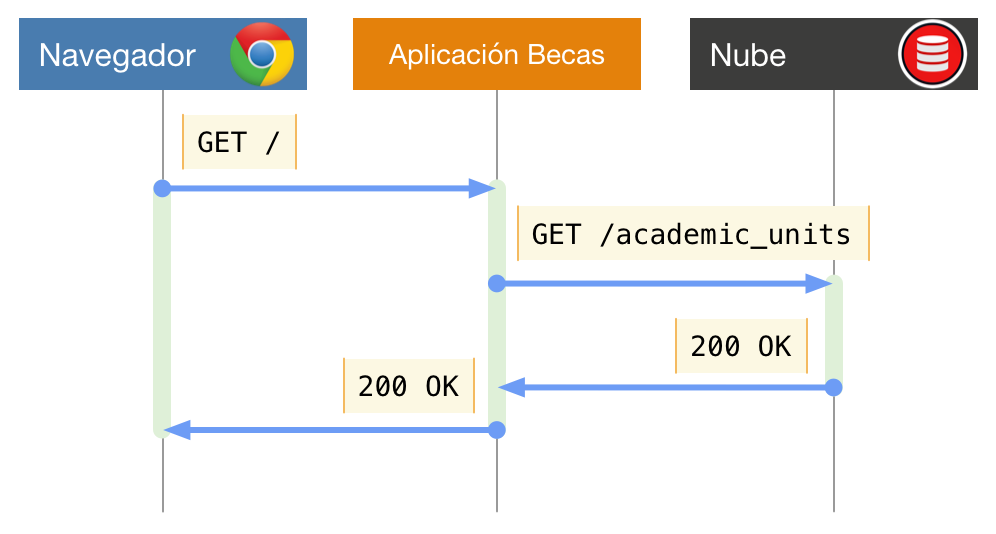
\includegraphics[width=\linewidth]{src/images/01-capitulo-1/ejemplo-rest-becas.png}
  \caption{Interacciones involucradas en el listado de becas por Unidad Académica}
  \label{fig:ejemplo-rest-becas}
\end{figure}

En la sección \ref{standard:rest} realizaremos el desarrollo pertinente de la definición de la arquitectura de aplicaciones distribuidas \gls{acro:rest} que Fielding publicó, dando de esa forma un marco teórico adecuado a las definiciones de nuestra nueva arquitectura para la nube de servicios.


\paragraph{El diseño final: el Integrador}

Luego de analizar las posibilidades que brindaba el uso de los principios \gls{acro:rest} en detalle, realizamos el primer diseño de cómo quedarían definidos los distintos servicios o \gls{term:endpoint} y decidimos darle un nombre: el \textit{Integrador}, una mezcla entre título de historieta\footnote{En cierto modo, nos recuerda historietas como Castigador (\eng{The Punisher}, de \eng{Marvel Comics}) – \url{https://es.wikipedia.org/wiki/Punisher}} y \eng{Terminator}, que nos acompaña hasta el día de hoy cuando hacemos referencia a la aplicación \textit{detrás} de la nube de servicios.

Realizando un enfoque más pragmático que correcto para el diseño, definimos servicios que retornan documentos \gls{lang:json} para cada una de las entidades que se podían consultar sin realmente analizar si serían realmente útiles, o si siquiera se accederían alguna vez. Fue de esta forma que la \gls{acro:api} se compuso de los más de 100 \gls{term:endpoint} que tiene hoy, que no siguen una misma línea en su diseño,  no tienen una estructura estándar de respuesta, y de los cuales efectivamente se usa tan solo el 46\%\footnote{Esta cifra surge de los datos que tenemos en nuestra herramienta de analíticas. De los 105 servicios que existen, 56 no registran accesos en el último año.}. En el \nameref{anexo:endpoints-nube-actual} listamos todos los servicios provistos por la nube para utilizar de referencia.

Sin entrar en detalles sobre cada \gls{term:endpoint}, el diseño existente muestra la falta de consistencia general en la definición de las \glspl{acro:url}, la sobrecarga de niveles de anidamiento en servicios como el que devuelve las materias del plan de estudios de una carrera de una Unidad Académica\footnote{\lstinline$/api/academic_unit/:id/career/:career_id/career_programme/:career_programme_id/career_subject.json$} que anida esos 3 niveles para mostrar la información, aunque los identificadores únicos de cada elemento podrían usarse, en una estructura más plana, para acceder directamente al último nivel, algo así como \lstinline$/api/career_programme/:career_programme_id/career_subject.json$ y así simplificar las \glspl{acro:url}.

Estos problemas sumados a la falta de documentación sobre cómo usar los diferentes servicios, qué parámetros reciben y qué estructura tiene la respuesta cada uno, hacen más complejo el uso de esta \gls{acro:api} tanto para desarrolladores que la venimos utilizando hace tiempo, como para nuevos integrantes del equipo a los que queremos sumar a alguna aplicación que haga uso de estos servicios.

\paragraph{El Integrador: implementación}

La nube de servicios, como aplicación, fue un desarrollo más realizado en PHP 5 y el framework \gls{fw:symfony} 1.4, utilizando MySQL como motor para las 5 bases de datos que utiliza para proveer la información:

\begin{itemize}
  \item Una base de datos donde se almacena información propia de la aplicación: tokens de acceso, estadísticas de acceso, información de clientes de la \gls{acro:api}.

  \item Una segunda base de datos para los datos de referencia de los que ya hemos hablado (tipos de documento, países, etcétera).

  \item Una tercera base en la que se mantiene actualizada la información que nos llega desde la oficina de Liquidaciones del CeSPI, la cual se transforma mediante procesos \gls{acro:etl}\footnote{Técnica que se utiliza para tomar datos de una o múltiples fuentes de información, modificarla y cargarla en una o más almacenes de datos. En nuestro caso utilizamos la herramienta Kettle de la versión de comunidad de la suite Pentaho para transformar los datos fuente, que nos llegan en archivos de texto plano, en inserciones normalizadas en nuestra base de datos MySQL.}\cite{paper:etl} para normalizarla antes de guardarla en esta base de datos.

  \item Una cuarta para la información que proviene de los SIU Guarani de las distintas Unidades Académicas, la cual es actualizada directamente por el grupo de Sistemas Académicos del {\cespi}.

  \item Y una quinta base de datos donde se unifican y mezclan los datos de las últimas 3 bases datos mencionadas, de manera tal que se logre una trazabilidad de la persona como un todo a lo largo de su \textit{vida en la UNLP}, ya sea como alumno, docente o no docente.
\end{itemize}

La aplicación se realizó sin considerar algunos aspectos claves para mejorar la \eng{performance} del lado de los clientes de la \gls{acro:api}, como puede ser utilizar cabeceras de \eng{caching}, compresión de respuestas, utilizar \eng{caches} compartidas y otras estrategias que desarrollaremos más en detalle como parte de nuestro análisis para el futuro de la nube de servicios.

Para las \gls{term:aplicacionessatelitales}, se realizó un \eng{plugin} de \gls{fw:symfony} que abstraía en clases y objetos la mayoría de los servicios existentes, implementando cierto mecanismo de \eng{caching} local a cada aplicación. Este mecanismo ayudó drásticamente a mejorar los tiempos de respuesta de las aplicaciones, con casos en que presentar una página al usuario tomaba alrededor de 20 segundos sin \eng{caching} y menos de 5 segundos con él. Pero por tratarse de decisiones realizadas meramente del lado de las aplicaciones cliente, existían situaciones en las que la información almacenada en esa \eng{cache} local quedaba desactualizada (\eng{stale}, en inglés) con respecto a lo que la \gls{acro:api} devolvía como el dato actual (\eng{fresh}, en inglés), por lo que en algunos casos se debió implementar un mecanismo manual de vaciado de \eng{cache} para subsanar estas situaciones.

En resumen: la implementación fue adecuada y funcional para las necesidades del momento, pero con el tiempo esas necesidades y, principalmente, la tecnología fueron cambiando, lo cual fue acrecentando gradualmente la necesidad de un nuevo análisis y replanteo para la solución actual.


\subsubsection{Cuarta iteración: este trabajo}
\label{nube:etapa4}

Mucha agua ha pasado bajo el puente desde que implementamos la versión actual de la nube de servicios de la UNLP, y varios han sido los cambios que el paso de estos 4 años nos ha dejado: pasamos de ser un equipo de alrededor de 8 personas en que todos nos dedicábamos a desarrollar aplicaciones web en PHP con el framework \gls{fw:symfony}, algunos toques de JavaScript para la interfaz de usuario y bases de datos MySQL, a ser un equipo de 17 personas que desarrolla aplicaciones en el lenguaje Ruby, con \gls{fw:rails} y \gls{fw:sinatra} como \eng{frameworks} web de cabecera, realizando algunas pequeñas aplicaciones meramente en JavaScript, que ha reescrito en Ruby varias de las aplicaciones realizadas en PHP y mantiene activamente aquellas desarrolladas en \gls{fw:symfony} que aún no se han migrado, utilizando bases de datos MySQL mayoritariamente y en algunos casos combinándolas con bases de datos \gls{db:nosql} y almacenes clave-valor en memoria, como \gls{db:redis} o \gls{db:memcached}. A modo de referencia, en el  \nameref{anexo:detalle-clientes} detallamos las aplicaciones que actualmente estamos manteniendo y desarrollando.

Estos cambios han traído aparejada la implementación de un cliente desarrollado en Ruby para integrarlo, de la misma forma que lo hicimos en el caso de las aplicaciones PHP, en las aplicaciones basadas en \gls{fw:rails} y \gls{fw:sinatra}. Este fue otro caso más donde las limitaciones del Integrador actual debieron ser sorteadas mediante la adición de lógica del lado del cliente:

\begin{itemize}
  \item Las aplicaciones cliente desarrolladas en Ruby implementan una cache condicional basada en \gls{db:redis} o en archivos del filesystem (según disponibilidad, y en ese orden de prioridad), que almacena las respuestas a los requerimientos por un tiempo determinado\footnote{La posibilidad de especificar el tiempo por el cual se desea guardar la copia en cache (el \gls{acro:ttl}) fue agregada recién en abril de 2015, es decir que antes se almacenaban indefinidamente las copias en \eng{cache}, lo que para los casos en que se usaba el sistema de archivos como almacenamiento esto representaba un potencial problema de crecimiento sin tope de los archivos utilizados para la cache.} e intenta subsanar la falta de directivas de cabeceras de parte de la \gls{acro:api} de servicios.

  \item Al no tener un estándar para la estructura de las respuestas, la lógica de hidratación de estos documentos \gls{lang:json} para convertirlos en objetos del dominio de las aplicaciones es excesivamente costosa en términos de \eng{performance} y tiene varios chequeos que podrían evitarse si se normalizaran y estandarizasen las respuestas.

  \item La falta de documentación nos ha obligado en ocasiones teniendo que hacer una suerte de ingeniería inversa de las respuestas para entender relaciones entre datos.
\end{itemize}

Otro gran problema es la dificultad para escalar que tiene la arquitectura actual. La aplicación web que atiende los pedidos a la nube y sus 5 bases de datos viven en una misma máquina virtual, lo cual puede ser hasta cierto punto conveniente para tener un mantenimiento y administración centralizados, pero esto acota en gran medida la posibilidad de poner rápidamente en funcionamiento nuevas instancias de la \gls{acro:api} que puedan balancear proporcionalmente la carga ante la creciente demanda que tiene por parte de las aplicaciones cliente. Este único punto de falla también es un potencial riesgo en caso de intrusiones o caídas de cualquier índole: fallas eléctricas, de red, de disco o errores humanos a la hora de realizar el mantenimiento de ese equipo virtual. Las tecnologías que utiliza ya no son mantenidas por sus desarrolladores: PHP 5.3 alcanzó su fin de mantenimiento (o \eng{end of life}, como la comunidad de PHP lo denomina) el 14 de agosto de 2014\footnote{Cf. \url{http://php.net/eol.php}} y \gls{fw:symfony} 1.4 dejó de ser mantenido en Noviembre de 2012\footnote{Cf. \url{http://symfony.com/blog/symfony-1-4-end-of-maintenance-what-does-it-mean}}, lo cual implica que en cierto modo la aplicación puede eventualmente ser víctima de nuevas vulnerabilidades que se descubran a esa rama del desarrollo y que ya no serán solucionadas.

Todos estos cambios y problemas motivan el presente trabajo, en el cual analizaremos las posibilidades que ofrece una \gls{acro:api} diseñada desde el comienzo con el nivel más alto\footnote{Así define Leonard Richardson el conjunto de requerimientos para alcanzar un servicio que cumpla realmente con todos los principios que Roy Fielding definió para una \gls{acro:api} \gls{acro:rest}, y define que \gls{acro:hateoas} es el requerimiento de nivel 3 para alcanzar la pureza de \gls{acro:rest}. – \url{http://www.crummy.com/writing/speaking/2008-QCon/act3.html} y claramente analizado por Martin Fowler en \url{http://martinfowler.com/articles/richardsonMaturityModel.html}} de adhesión a \gls{acro:rest} posible (\gls{term:hypermedia}), basándonos en estándares ya establecidos en lugar de intentar reinventar la rueda y definir el nuestro propio para las respuestas \gls{lang:json}, pensando en aprovechar las posibilidades de caching que ofrecen las distintas capas del diseño, e intentando descentralizar la información de manera tal que se elimine el único punto de falla que existe en la actualidad y que nos permita escalar horizontalmente en cantidad de instancias de la nube de manera transparente y poco costosa.

  \newpage
  %   - Capítulo II
  \section{Capítulo II}
  \textbf{\textit{TODO}}

  \newpage
  %   - Capítulo III
  \section{Capítulo III}
  \textbf{\textit{TODO}}

  \newpage
  %   - Capítulo IV
  \section{Capítulo IV}
  \textbf{\textit{TODO}}

  \newpage

  %   - Sin organizar aún
  \section{\textit{SIN ORGANIZAR}}
  \subsection{REpresentational State Transfer (REST)}
\label{standard:rest}

En el capítulo 5 de su tesis doctoral, Roy Fielding define el estilo de arquitectura de las aplicaciones web o, en términos más generales, de los sistemas distribuidos basados en hypermedia. Esta arquitectura, a la que denomina \gls{acro:rest}, está presentada como una derivación a partir de las restricciones de interacción que impone, partiendo de un estilo base sin restricciones, al que va agregando otras limitaciones hasta llegar a definir el modelo \gls{acro:rest}. Al realizar la caracterización de esta forma, Fielding logra de forma natural analizar qué propiedades surgen a partir de cada restricción aplicada.


\subsubsection{Derivación de REST}
\label{standard:rest:derivacion}

En esta sección resumiremos el proceso de derivación que realiza Fielding para, a partir de un estilo base al que se le van agregando restricciones o propiedades, llegar a definir el estilo de aplicaciones distribuidas \gls{acro:rest}.

\paragraph{Estilo base}

La derivación de \gls{acro:rest} parte de un estilo de sistemas distribuidos base en el que no existen restricciones ni límites entre los elementos que lo componen.


\paragraph{Cliente-Servidor}

Las primeras restricciones aplicadas al estilo base son aquellas del estilo Cliente-Servidor\cite[Sec.~3.4.1]{tesis:fielding}, en el que un componente Servidor ofrece un conjunto de servicios y escucha peticiones a los mismos, mientras que un componente Cliente realiza solicitudes indicando que desea se realicen esos servicios a través de un \textit{conector}. Ante la recepción de la petición, el Servidor rechaza o realiza lo solicitado y envía en retorno una respuesta al Cliente.
Estas adiciones al conjunto, inicialmente vacío, de limitaciones beneficia al principio de separación de responsabilidades y permite que los componentes Cliente y Servidor evolucionen independientemente, habilitando a una gran escalabilidad de esta arquitectura.


\paragraph{Sin estado}

Tomando ahora como base el estilo Cliente-Servidor, se agrega la restricción de que el Servidor no puede contener información del estado de la sesión\cite[Sec.~3.4.3]{tesis:fielding}: las peticiones realizadas al Servidor deben incluir toda la información necesaria para reflejar el estado actual de la comunicación.

De esta forma, se obtienen nuevas propiedades positivas para el estilo en evolución: visibilidad, confiabilidad y escalabilidad. El sistema gana en visibilidad ya que dado un requerimiento, no se necesita ningún dato adicional para conocer su naturaleza; es más confiable ya que recuperarse, al menos en forma parcial, de un fallo implica simplemente retomar el requerimiento que falló; y la falta de información de estado del lado del Servidor, simplifica su implementación y permite escalar fácilmente instancias del servidor que puedan atender esos requerimientos. Como contrapunto, este conjunto de restricciones tiende a ser penalizado con una performance disminuida sobre las comunicaciones de red, al necesitar incluir y repetir la información del estado en cada petición.


\paragraph{Cache}

A fin de disminuir las penalidades en performance que trae aparejadas el modelo Sin estado definido en el apartado anterior mejorando la eficiencia en el uso de la red, se agrega la restricción del uso de Cache de respuestas\cite[Sec.3.4.4]{tesis:fielding}. La Cache funciona como intermediario entre el Cliente y el Servidor, encargándose de almacenar las respuestas \textit{marcadas como cacheables} por el Servidor de manera tal que peticiones posteriores equivalentes a una anterior con estas características puedan obtener la misma respuesta sin llegar a consultar al Servidor.

Esta adición puede eliminar parcial o inclusive completamente algunas interacciones entre Cliente y Servidor, mejorando la eficiencia de uso de recursos de red y la performance perceptible desde el punto de vista del usuario.

Si bien este punto de la tesis de Fielding hace referencia a la Cache únicamente del lado del Cliente, nosotros tomaremos una postura más general, en la que la Cache puede ubicarse tanto del lado del Cliente como del Servidor, para poder incluir en este estilo a las Cache compartidas o Cache de \eng{Gateway}. Éste tipo de caches funcionan más cercanas al Servidor y permiten que, sin importar si los clientes implementan mecanismos de caching de respuestas, se reduzca la cantidad de requerimientos que efectivamente llegan a ser procesadas por el Servidor, al cachear las respuestas marcadas como cacheables e interceptar las peticiones que los clientes realizan, respondiendo con las respuestas cacheadas que dispongan en caso de aplicar. Las caches de Gateway también permiten alivianar la carga del Servidor cuando múltiples clientes realizan peticiones repetitivas.

El posible problema de agregar la Cache al estilo de arquitectura anterior es que existe la posibilidad de que un recurso cacheado esté desactualizado (\eng{stale}, como se lo referencia comúnmente en inglés) con respecto a la respuesta que el Servidor proveería si esa petición le llegase.


\paragraph{Interfaz uniforme}

Uno de los puntos centrales que aporta \gls{acro:rest} en su definición es la importancia que da a la necesidad de una interfaz uniforme entre los componentes de la arquitectura. Mediante la generalización del diseño del conector utilizado en las comunicaciones y la forma en que se transfiere la información, se simplifica la arquitectura general, a costo de no hacer el uso más eficiente posible de la forma de transmitir los datos, al hacerlo de una forma estandarizada y no una hecha a medida acorde a la información que se necesita intercambiar. La interfaz normalizada que \gls{acro:rest} define está pensada para lograr eficiencia al transferir datos \gls{term:hypermedia} - como es el caso de la web - pero puede resultar subóptima para otro tipo de interacciones. La forma de lograr esta uniformidad es a partir de restricciones: un mecanismo unívoco para la identificación de recursos, la manipulación de estos recursos mediante representaciones, el uso de mensajes autodescriptivos y, principalmente, \gls{acro:hateoas}: el uso de \gls{term:hypermedia} como el motor del estado de la aplicación.


\paragraph{Sistema en capas}

La siguiente limitación que agrega la derivación en la que Fielding define \gls{acro:rest} es la de un sistema desarrollado en capas. Este estilo permite que la arquitectura se componga de capas jerárquicas que se conectan unas a otras de forma tal que un componente no pueda tener conocimiento más allá de la capa con la que está interactuando. Esta forma de concebir las interacciones permite que las capas abstraigan de la complejidad y la posible heterogeneidad de los sistemas que ocultan, y que se uso simplifique la escalabilidad de los sistemas al poder agregar capas que funcionen como balanceadores de carga.


\paragraph{Código bajo demanda}

Por último, se agrega la restricción que identifica la forma de comunicación de la web: los Clientes son entidades con una funcionalidad general, capaces de interpretar el código que el Servidor le envía como respuesta a sus peticiones, a partir del cual obtienen el conocimiento específico. La forma en que se transmite este \eng{know-how} al Cliente es mediante \eng{scripts}\footnote{En su especificación, Fielding además incluye los applets como medios, pero los obviaremos por tratarse de una tecnología en desuso en la actualdad, reemplazada y superada ampliamente por JavaScript.} que extienden esa funcionalidad básica, beneficiando a la extensibilidad del sistema general, pero reduciendo la visibilidad, por lo cual esta restricción es opcional.


\subsubsection{Elementos de la arquitectura REST}
\label{standard:rest:elementos}

\paragraph{Elementos de datos}

\gls{acro:rest} basa las interacciones (la transmisión de la información) en el conocimiento compartido de los tipos de datos a través de la inclusión de metadatos. Los componentes se comunican transfiriendo los recursos utilizando formatos de representación estandarizados, elegidos acorde a lo solicitado por el receptor y la naturaleza del recurso. De esta forma, la información se compone de los siguientes elementos de datos:

\begin{itemize}
  \item \textbf{Recursos e identificadores de recursos:} los recursos son la principal abstracción de \gls{acro:rest}, y hacen referencia a un conjunto de propiedades de una entidad en un momento dado del tiempo. Esas propiedades pueden ser representaciones de recursos o identificadores de recursos, cuya semántica es lo que efectivamente diferencia un recurso de otro. \gls{acro:rest} utiliza los identificadores de recursos en la forma en que la web utiliza \glspl{acro:url} y \glspl{acro:urn} para referenciar recursos utilizando \gls{term:hypermedia}.

  \item \textbf{Representaciones:} los componentes las utilizan para operar sobre el estado actual de un recurso y transmitirla entre sí. Una representación consiste de datos, metadatos para describirlos y, en algunos casos, metadatos para describir a los anteriores (también llamados datos de control), por ejemplo para validar la integridad de un mensaje. Los metadatos tienen la forma clave-valor, donde las claves obedecen al estándar que define la estructura y semántica del valor. La forma de describir la estructura de la información se llama \eng{media type}.
\end{itemize}


\paragraph{Conectores}

El estilo de arquitectura \gls{acro:rest} utiliza diferentes tipos de conectores para encapsular el acceso a los recursos y la transferencia de sus representaciones. Estos tipos se agrupan en:

\begin{itemize}
  \item \textbf{Clientes:} junto a los servidores, son el tipo principal de conectores. Inician las comunicaciones al enviar una solicitud a un servidor.

  \item \textbf{Servidores:} esperan recibir (``escuchan'') solicitudes (``conexiones'') de los clientes, a las que responden a fin de dar acceso a sus servicios.

  \item \textbf{Caches:} pueden encontrarse en conexión a un cliente o un servidor. Su función es almacenar respuestas marcadas como cacheables para evitar realizar subsiguientes peticiones similares.

  \item \textbf{Resolvers:} traducen identificadores de recursos a la información efectiva de red necesaria para conectar los distintos componentes involucrados.

  \item \textbf{Túneles:} permiten realizar conexiones entre componentes que crucen alguno de los límites impuestos por la arquitectura en capas, generando comunicaciones directas entre componentes que de otra forma no podrían tener contacto.
\end{itemize}

Los conectores tienen una interfaz abstracta para establecer las comunicaciones entre los componentes, lo cual oculta los detalles del funcionamiento de conexión interno, separa las responsabilidades y permite que la implementación de cualquier parte del sistema sea remplazada sin afectar al resto de las entidades involucradas. En su funcionamiento, utilizan dos conjuntos de elementos en los mensajes, uno para el de la solicitud y otro para el de la respuesta. El primero consiste en datos de control de la solicitud (por ejemplo, para definir el formato en que se desea el recurso), un identificador de recurso (para indicar a qué recurso se desea acceder), y una representación opcional (por ejemplo, los datos con los que se quiere actualizar una entidad). El conjunto de elementos utilizado en las respuestas se compone de datos de control para la respuesta (como información necesaria para alojar la respuesta en una cache), opcionalmente metadatos del recurso (como \eng{links} relacionados al recurso), y una representación (por ejemplo, el recurso solicitado en sí), también opcional.


\paragraph{Componentes}

Las partes que conforman la arquitectura de los sistemas \gls{acro:rest} se pueden clasificar acorde a su rol en las interacciones en:

\begin{itemize}
  \item \textbf{\eng{User agent}:} utiliza un conector cliente para enviar una solicitud, iniciando una comunicación, y luego espera una respuesta, la cual al llegar finalizará la interacción.

  \item \textbf{\eng{Proxy}:} componente intermediario que funciona más cercano al lado del cliente, encapsulando la interfaz hacia otros servicios y, opcionalmente, brindando otras funcionalidades como traducción de información, mejoras de performance y medidas adicionales de seguridad. Funciona con conectores cliente y servidor para transmitir los mensajes (solicitudes y respuestas) que llegan a él.

  \item \textbf{\eng{Gateway} o \eng{Reverse proxy}:} otro componente intermediario, este más cercano al servidor de origen, también encapsula servicios y puede brindar traducción de los datos que por él circulan, optimizaciones en la performance y realizar acciones para mitigar posibles problemas de seguridad. Al igual que un \eng{proxy}, funciona como cliente y servidor a la vez, reenviando la información que por él pase.

  \item \textbf{Servidor de origen:} utiliza un conector de servidor para recibir solicitudes dirigidas a sus recursos. Las peticiones que le llegan obedecen a una estructura jerárquica que define cómo acceder a los servicios que provee.
\end{itemize}


\subsubsection{REST aplicado a nuestro trabajo}
\label{standard:rest:aplicado}

\textbf{\textit{@ncuesta: Estaría bueno cerrar este tema con un breve análisis de cómo REST se aplica a nuestro trabajo, para dar un ejemplo concreto de todo lo definido antes. Utilizar como referencia el capítulo 6 de Fielding: https://www.ics.uci.edu/~fielding/pubs/dissertation/evaluation.htm}}

\begin{figure}
  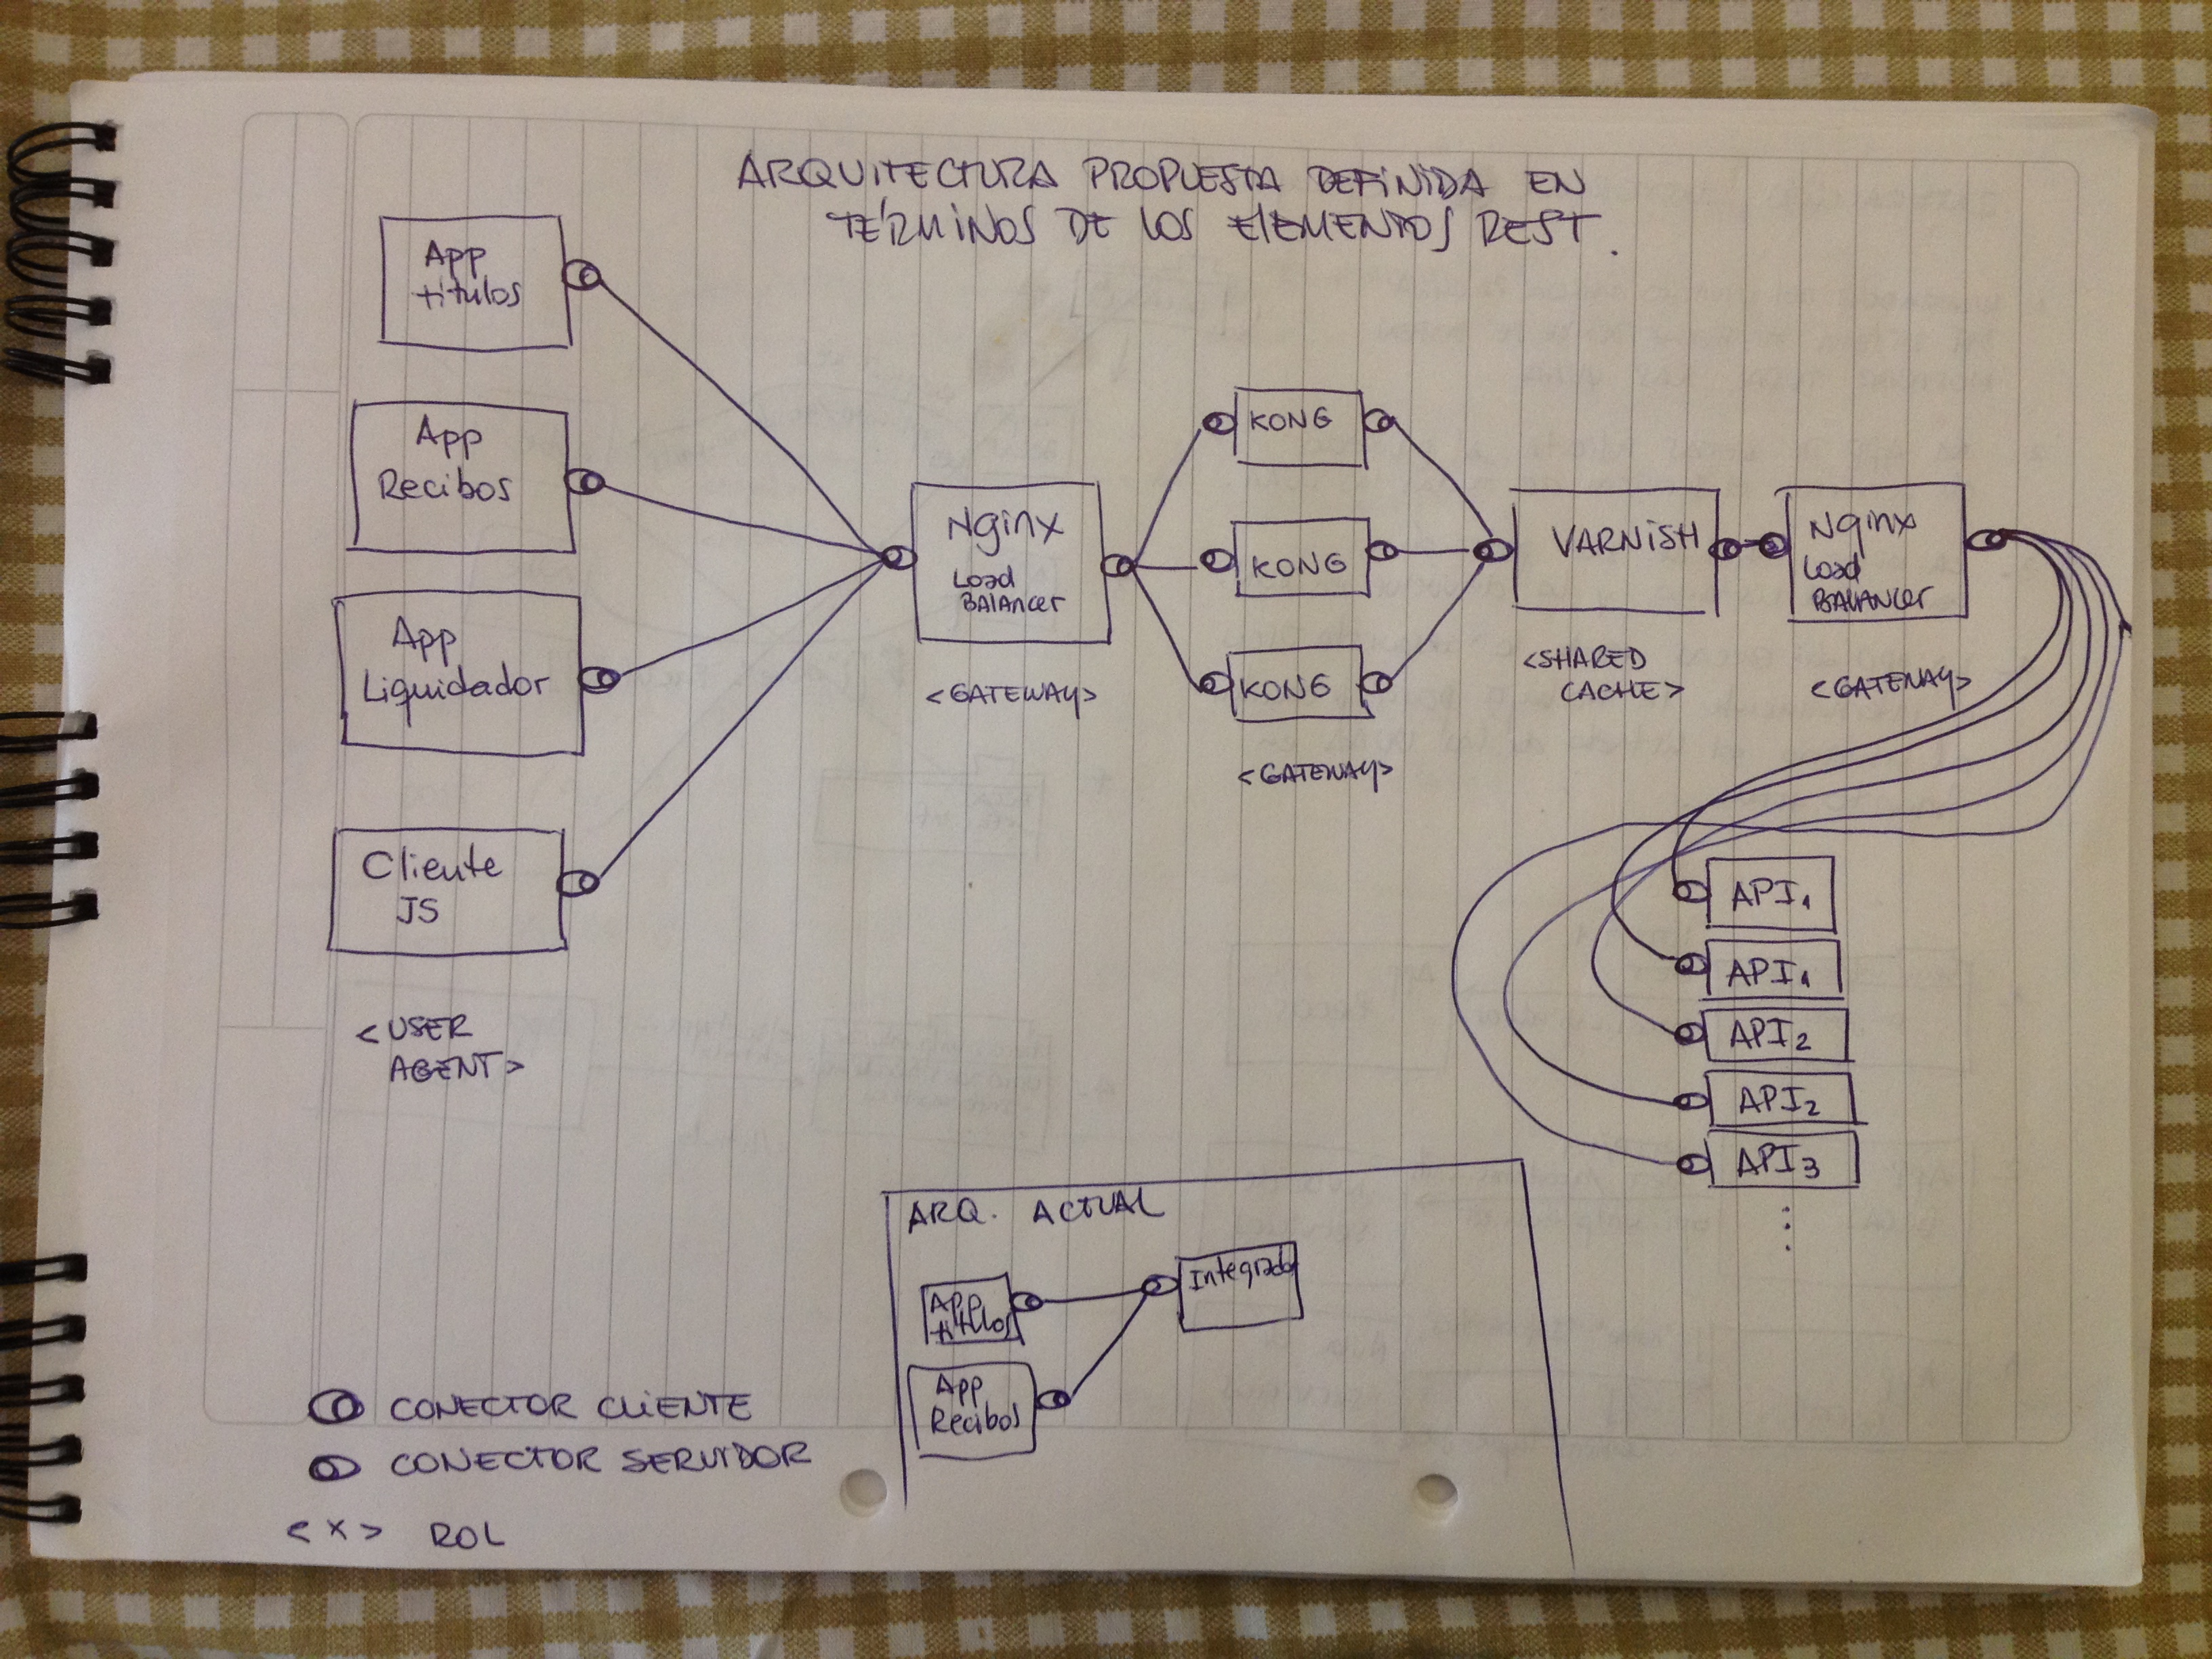
\includegraphics[width=\linewidth]{src/images/sin-organizar/nueva-arq-segun-rest.jpg}
  \caption{Visión \gls{acro:rest} de la nueva arquitectura propuesta.}
  \label{fig:ejemplo-rest-nueva-arquitectura}
\end{figure}

  \newpage

  % Apéndice
  \appendix
  \newpage
  %   - Anexo I: Detalle de las aplicaciones cliente de la nube
  \section{Anexo I}
\label{anexo:detalle-clientes}

\subsection{Aplicaciones cliente de la nube de servicios de la UNLP}

Como ya hemos mencionado antes, la nube de servicios de la {\unlp} es el almacén de datos de referencia y de dominio general de las aplicaciones de uso interno de la UNLP que desarrollamos en nuestra oficina. En esta sección daremos un marco más concreto en referencia a qué aplicaciones la utilizan de manera que el lector pueda comprender en detalle el alcance y las interacciones existentes que movilizan el rediseño motivo del presente trabajo.

Por último, detallaremos las dependencias existenes entre las distintas aplicaciones y la nube de servicios, indicando qué \glspl{acro:api} utiliza cada una.


\subsubsection{Albergue Universitario}
\label{anexo:detalle-clientes:albergue}

Esta aplicación permite la gestión administrativa, de personal y de alumnos alojados en el Albergue Universitario de la {\unlp}. Los usuarios del sistema son el personal administrativo, del comedor y de Guardia Edilicia que desempeñan sus tareas en esa institución, permitiéndoles manejar las entradas y salidas de los alumnos, planificar las comidas acorde a la cantidad de comensales, y llevar un registro detallado de las actividades que por reglamento deben realizar los alumnos como parte de la beca que les permite residir en el albergue.

Es una aplicación desarrollada en \gls{fw:rails} versión 3, que actualmente se encuentra en etapa de mantenimiento correctivo de errores.


\subsubsection{Asociador}
\label{anexo:detalle-clientes:asociador}

El Asociador de documentos es una aplicación desarrollada para el uso conjunto entre el área de Digitalización de documentos del {\cespi} y la Dirección de Salud de la {\unlp}. Su objetivo es permitir que ése área suba en formato PDF las carpetas médicas históricas que digitaliza y luego las asocie a los agentes de la {\unlp}, de modo tal que el personal de la Dirección de Salud pueda consultar en línea dichas carpetas sin necesidad de contar con una oficina llena de biblioratos con las carpetas médicas otorgadas en los últimos 20 años en soporte papel.

Esta aplicación está desarrollada en \gls{fw:rails} versión 3, y actualmente se encuentra en etapa de mantenimiento correctivo de errores.


\subsubsection{Becas UNLP}
\label{anexo:detalle-clientes:becas}

La aplicación de Becas de la {\unlp} posee dos partes principales: una pública donde los alumnos (y futuros alumnos) de la Universidad pueden identificarse y solicitar algunas de las becas que la Universidad ofrece, y una privada accesible por personal de la Dirección de Becas que les permite realizar la asignación de las becas acorde a un órden de mérito que calcula el sistema, habilitar o deshabilitar becas de entre la oferta existente y agregar nuevas para que sean publicadas.

Está desarrollada en \gls{fw:symfony} versión 1.4, y actualmente se encuentra en etapa de mantenimiento correctivo de errores con soporte para nuevos requerimientos.


\subsubsection{Libretas Sanitarias}
\label{anexo:detalle-clientes:libretas}

Permite al personal de la Dirección de Salud la gestión de la información referente a las libretas sanitarias de los alumnos de la {\unlp}, la obtención de turnos y la consulta del estado de los trámites relacionados.

Se encuentra implementada con el \eng{framework} \gls{fw:rails} versión 3, y en este momento se encuentra bajo proceso de \gls{term:refactor} y migración a \gls{fw:rails} versión 4.


\subsubsection{Licencias Médicas}
\label{anexo:detalle-clientes:licencias}

La Dirección de Salud de la UNLP utiliza este sistema para gestionar las solicitudes de carpetas médicas, el tratamiento de esas solicitudes y el seguimiento de las eventuales licencias otorgadas a partir de ellas o las juntas médicas que pudieran surgir.

Esta aplicación fue desarrollada en \gls{fw:symfony} versión 1.2, y se encuentra en etapa de mantenimiento correctivo de errores. Tenemos planificada para la segunda mitad del año 2016 una reescritura de la aplicación para actualizar su \eng{stack} y extender su funcionalidad para brindar mejor soporte a situaciones no previstas en la versión actual, como por ejemplo permitir que los agentes de la {\unlp} soliciten en línea sus licencias, en lugar de tener que presentar en papel o telefónicamente los pedidos.


\subsubsection{Programa ``Mejor Aire''}
\label{anexo:detalle-clientes:mejor-aire}

Aplicación que gestiona las inscripciones de agentes de la UNLP al programa ``Mejor Aire'', una iniciativa de la Universidad para ayudar a dejar de fumar. Los inscriptos al programa participan semanalmente de reuniones de grupo y tienen controles periódicos para hacer un seguimiento de su evolución en el proceso. Mediante esta aplicación, los profesionales que llevan adelante el programa organizan los turnos, la asistencia a las reuniones y registran los chequeos realizados a cada inscripto.

Este sistema fue desarrollado utilizando \gls{fw:symfony} 1.2, y actualmente se encuentra en etapa de mantenimiento correctivo de errores.


\subsubsection{Proyectos de Extensión}
\label{anexo:detalle-clientes:extension}

El sistema actual de gestión de Proyectos de Extensión de la {\unlp} es el resultado de dos iteraciones de análisis de requerimientos e implementación, a partir de las cuales se depuraron las necesidades reales que la Secretaría de Extensión Universitario tenía para la versión \eng{on line} del proceso de presentación, acreditación, evaluación y adjudicación de los proyectos postulados para el programa de subsidio de proyectos de extensión de la Universidad Nacional de La Plata. La aplicación es utilizada por los directores y miembros de los proyectos para presentar sus propuestas, por los Secretarios de Extensión para avalar los proyectos presentados desde su Unidad Académica, por los integrantes de las comisiones evaluadoras para analizar y calificar las presentaciones, y por el personal de la Secretaría de Extensión para el otorgamiento final y seguimiento posterior de los proyectos subsidiados.

Este sistema fue reescrito en el año 2015, pasando de un desarrollo en \gls{fw:symfony} 1.1 a una aplicación totalmente renovada y con mucha más funcionalidad implementada utilizando el \eng{framework} \gls{fw:rails} versión 4. Se encuentra en desarrollo activo.


\subsubsection{Recibos de sueldo}
\label{anexo:detalle-clientes:recibos}

La aplicación de Recibos de sueldo permite a los agentes de la {\unlp} acceder de manera cómoda y a todo momento a sus recibos de sueldo, con la posibilidad de descargarlos para utilizarlos a su conveniencia, sin necesidad de acercarse a la oficina de Personal de su Dependencia para obtenerlos.

Esta aplicación también fue reescrita por completo en el año 2015, proceso mediante el cual pasó de ser un sistema \gls{fw:symfony} 1.4 a uno desarrollado con \gls{fw:rails} versión 4. Se encuentra en etapa de mantenimiento correctivo de errores e implementación de nuevos requerimientos, en caso que surjan.


\subsubsection{Responsables}
\label{anexo:detalle-clientes:responsables}

Este sistema centraliza la información que la oficina de Responsables de la {\unlp} gestiona para el seguimiento y la rendición de cuentas sobre el destino dado a los fondos que la Universidad posee. Registra todos los gastos imputados a las distintas partidas presupuestarias, cerciorándose que no existan inconsistencias entre los montos otorgados, su destino y el uso efectivo de los mismos.

Fue desarrollada con \gls{fw:rails} versión 3, y en la actualidad se encuentra en etapa de mantenimiento correctivo de errores.


\subsubsection{Acceso Único (SSO)}
\label{anexo:detalle-clientes:sso}

En el año 2015 se implementó de manera global la centralización de cuentas de usuario de los agentes de la {\unlp} para las aplicaciones que nuestra {\direccionDesarrollo} realiza, haciendo que cada persona disponga de una única cuenta que le permita acceder a aquellas aplicaciones que utilice para su labor diaria, así como también a sus datos personales y recibos de sueldo. Este proceso comprendió la creación de más de 5000 cuentas de usuario, la implementación de un proceso de autoregistro para los agentes y capacitaciones para los agentes de las oficinas de Personal de cada Dependencia en su uso.

Es una aplicación desarrollada en tres partes, dos de gestión (una para autogestión de cada usuario) y otra de administración general de los datos de usuarios, permisos y aplicaciones utilizando \gls{fw:rails} versión 4 y otra que implementa el estándar \gls{acro:saml} para proveer autenticación y autorización al resto de las aplicaciones. Se encuentra en mantenimiento correctivo de errores, con una planificación para extender su funcionalidad en el año 2016.


\subsubsection{Sueldos}
\label{anexo:detalle-clientes:sueldos}

La aplicación de Sueldos de la UNLP es una reimplementación completa del sistema que actualmente se encuentra en uso para liquidar los sueldos de la Universidad. Como aplicación, además de realizar el cálculo de la liquidación de sueldos, es el puntapié inicial para un sistema integral de gestión de recursos humanos de la {\unlp}. Este proyecto lleva alrededor de dos años en desarrollo y está planificado para ser puesto en producción en la primer mitad del año 2016.

Esta aplicación está desarrollada en \gls{fw:rails} versión 4, y se encuentra en desarrollo activo.


\subsubsection{Títulos}
\label{anexo:detalle-clientes:titulos}

Aplicación desarrollada para la Oficina de Títulos que digitaliza el proceso de solicitud de los títulos otorgados por la {\unlp} a sus alumnos, comprendiendo todas las etapas involucradas en el mismo desde la solicitud inicial hasta la entrega final del título en papel.

Este sistema fue desarrollado utilizando \gls{fw:rails} 3, se encuentra en mantenimiento correctivo de errores. Se tiene planificada su reescritura para el año 2016 debido a recientes cambios en el alcance inicialmente definido.


\subsubsection{Dependencias con la nube de servicios}
\label{anexo:detalle-clientes:dependencias-nube}

A continuación se presenta un cuadro que describe qué grupos de datos de los que provee la nube de servicios utilizan las aplicaciones enumeradas en este anexo.

En este cuadro se indica con un tilde ({\checkmark}) en qué grupos de \glspl{acro:api} depende cada aplicación, siendo los posibles grupos los siguientes:

\begin{itemize}
  \item \textbf{Ref} comprende las \glspl{acro:api} de datos de referencia.
  \item \textbf{Alumnos} abarca las \glspl{acro:api} de datos de alumnos de la UNLP.
  \item \textbf{Personal} referencia las \glspl{acro:api} de datos de agentes que trabajan en la {\unlp}.
  \item \textbf{Usuarios} indica que la aplicación usa las \glspl{acro:api} de datos de cuentas de usuarios registrados en el Sistema de Acceso Único.
\end{itemize}

\begin{table}[h!]
  %\begin{tabular*}{\textwidth}{ @{\extracolsep{\fill}} | p{0.4\textwidth} | m{0.15\textwidth} | m{0.15\textwidth} | m{0.15\textwidth} | m{0.15\textwidth} | }
  \begin{tabular*}{\textwidth}{ @{\extracolsep{\fill}} | p{0.39\textwidth} | c | c | c | c | }
    \hline
    \textbf{Aplicación}                           & \textbf{Ref} & \textbf{Alumnos} & \textbf{Personal} & \textbf{Usuarios} \\ \hline
    \nameref{anexo:detalle-clientes:albergue}     & {\checkmark} & {\checkmark}     &                   &                   \\ \hline
    \nameref{anexo:detalle-clientes:asociador}    & {\checkmark} &                  & {\checkmark}      &                   \\ \hline
    \nameref{anexo:detalle-clientes:becas}        & {\checkmark} & {\checkmark}     &                   &                   \\ \hline
    \nameref{anexo:detalle-clientes:libretas}     & {\checkmark} & {\checkmark}     &                   &                   \\ \hline
    \nameref{anexo:detalle-clientes:licencias}    & {\checkmark} &                  & {\checkmark}      &                   \\ \hline
    \nameref{anexo:detalle-clientes:mejor-aire}   & {\checkmark} &                  & {\checkmark}      &                   \\ \hline
    \nameref{anexo:detalle-clientes:extension}    & {\checkmark} & {\checkmark}     & {\checkmark}      & {\checkmark}        \\ \hline
    \nameref{anexo:detalle-clientes:recibos}      & {\checkmark} &                  & {\checkmark}      &                   \\ \hline
    \nameref{anexo:detalle-clientes:responsables} & {\checkmark} &                  &                   &                   \\ \hline
    \nameref{anexo:detalle-clientes:sso}          & {\checkmark} & {\checkmark}     & {\checkmark}      & {\checkmark}        \\ \hline
    \nameref{anexo:detalle-clientes:sueldos}      & {\checkmark} &                  & {\checkmark}      &                   \\ \hline
    \nameref{anexo:detalle-clientes:titulos}      & {\checkmark} & {\checkmark}     &                   &                   \\ \hline
  \end{tabular*}
  \caption{Dependencias de las aplicaciones con los servicios de la nube}
  \label{anexo:detalle-clientes:dependencias-nube:tabla}
\end{table}

\clearpage

  \newpage
  %   - Bibliografía
  \bibliographystyle{plain}
  \bibliography{src/bibliografia/mcarbone,src/bibliografia/ncuesta}
  \newpage
  %   - Glosario
  \printglossary[title={Glosario de términos}]
  \newpage
  %   - Lista de figuras
  \listoffigures
  \newpage
  %   - Lista de tablas
  \listoftables
\end{document}
